\documentclass{article}

\usepackage[T1]{fontenc}
\usepackage{polski}
\usepackage[utf8]{inputenc}

\usepackage{hyperref}
\usepackage[legalpaper, margin=1.2in]{geometry}

\usepackage{listings}
\usepackage[]{algorithm2e}

\title{AEM - Zadanie nr 5}
\author{Bartosz Sobkowiak 125342 Joanna Świda 138675}
\date{25.05.2020}

\usepackage{natbib}
\usepackage{graphicx}

\begin{document}

\maketitle
\section{Opis zadania}

    Rozważany problem to zmodyfikowana wersja problemu komiwojażera. Dany jest zbiór wierzchołków i macierz symetrycznych odległości między nimi. Zadanie polega na implementacji czterech metod - multiple start local search oraz dwóch rodzajów iterated local search, a także hybrydowego algorytmu ewolucyjnego i porównanie ich ze sobą.

\section{Pseudokod}

\vspace{10mm}

\begin{algorithm}[H]
     \KwData{zbiór wierchołków, macierz odległości pomiędzy wierzchołkami}
     \KwResult{najlepsze rozwiązanie}
     
    wygeneruj losowe rozwiązania w liczbie 20\\
    wyznacz ścieżki na podstawie algorytmu localSearch \\
    \While{dopóki nie przekroczono czasu}{
        wyznacz losowo indeksy rodziców do krzyżowania przy pomocy modułu random \\
        wykonaj krzyżowanie (crossover) - po 50\% wierzchołków z każdego rozwiązania \\
        wykonaj mutacje wierzchołków (6) w sposób losowy \\
        sprawdź czy ścieżka jest cyklem, jeśli nie, to popraw w sposób zachłanny \\
        \textbf{IF:} jeśli któreś rozwiązanie po wprowadzonych zmianach jest lepsze - zapisz jako najlepsze znalezione do tej pory rozwiązanie, wybierz też grupę najlepszych rozwiązań i przekaż dalej do następnego pokolenia \\
            }
            \textbf{return:} najlepsze rozwiązanie \\ \\
            
            
\caption{Steady State - Evolutionary}
\end{algorithm}

\vspace{10mm}

\section{Wyniki obliczeń i wizualizacje}

\begin{table}[h!]
\centering
\begin{tabular}{ |c|c|c|c|c|c| } 
 \hline
 Zbiór & Wersja & Typ & Min & Avg & Max \\ 
  \hline
 kroA$_{200}$ & ILS & 1 & 15279 & 17071 & 18271  \\ 
  \hline
 kroA$_{200}$ & ILS & 2 & 14142 & 14814 & 15466 \\ 
 \hline
 kroA$_{200}$ & MSLS & - & 16013 & 16935 & 18800 \\
  \hline
 kroA$_{200}$ &  \textbf{Evol} & - & 14695 & 14852 & 15002 \\
  \hline
 kroB$_{200}$ & ILS & 1 & 15867 & 17068 & 18062 \\ 
  \hline
 kroB$_{200}$ & ILS & 2 & 14639 & 15147 & 15687 \\ 
 \hline
 kroB$_{200}$ & MSLS & - & 16631 & 16947 & 18348 \\
  \hline
 kroB$_{200}$ &  \textbf{Evol} & - & 14390 & 14750 & 15301 \\
 \hline
\end{tabular}
\caption{Wartości rozwiązań}
\end{table}

\begin{table}[h!]
\centering
\begin{tabular}{ |c|c|c|c|c|c| } 
 \hline
 Zbiór & Wersja & Typ & Min & Avg & Max \\ 
  \hline
 kroA$_{200}$ & ILS & 1 & 200.0444 & 200.0628 & 200.1011 \\
  \hline
 kroA$_{200}$ & ILS & 2 & 200.118 & 200.1526 & 200.2765 \\
 \hline
 kroA$_{200}$ & MSLS & - & 200.013 & 200.126 & 201.098 \\
  \hline
 kroA$_{200}$ & \textbf{Evol} & - & 200.9137 & 200.3126 & 201.1998 \\
  \hline
 kroB$_{200}$ & ILS & 1 & 200.0407 & 200.0598 & 200.1157 \\
  \hline
 kroB$_{200}$ & ILS & 2 & 200.003 & 200.0487 & 200.0996 \\
 \hline
 kroB$_{200}$ & MSLS & - & 200.1207 & 200.1581 & 201.1457 \\
 \hline
 kroB$_{200}$ &  \textbf{Evol} & - & 200.2607 & 200.8331 & 201.9237 \\
 \hline
\end{tabular}
\caption{Czasy trwania}
\end{table}

Średnia liczba iteracji lokalnego przeszukiwania dla ILS wynosiła 483 dla ILS2 (min:471 max:499 ) i 421 dla ILS1 (min:401 max:446).  \\

\begin{figure}[h!]
  \centering
  \begin{minipage}[b]{0.8\textwidth}
    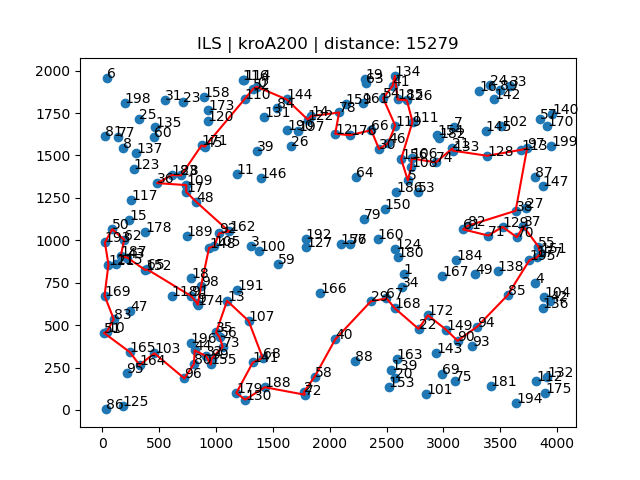
\includegraphics[width=\textwidth]{ils_kroA200.png}
  \end{minipage}

  \begin{minipage}[b]{0.8\textwidth}
    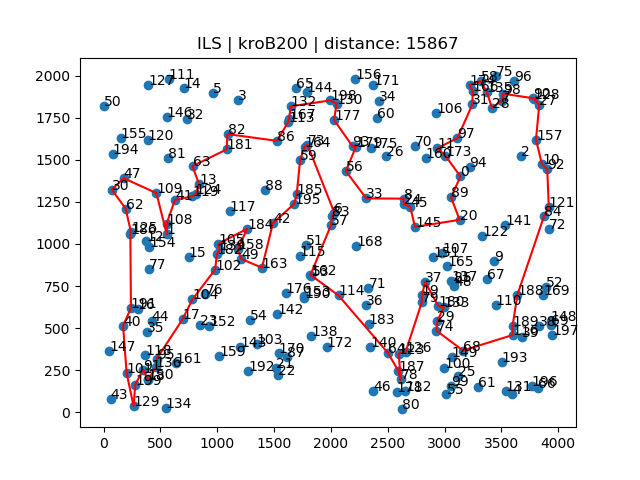
\includegraphics[width=\textwidth]{ils_kroB200.png}
  \end{minipage}
  
\end{figure}
    
\begin{figure}[h!]
    \centering
  \begin{minipage}[b]{0.8\textwidth}
    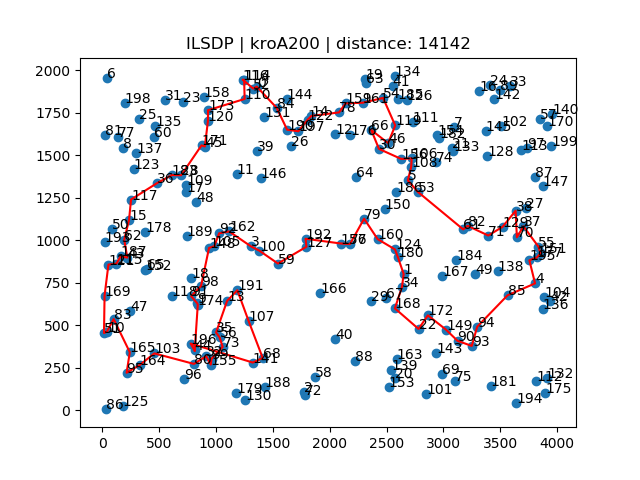
\includegraphics[width=\textwidth]{ilsdp_kroA200.png}
  \end{minipage}

  \begin{minipage}[b]{0.8\textwidth}
    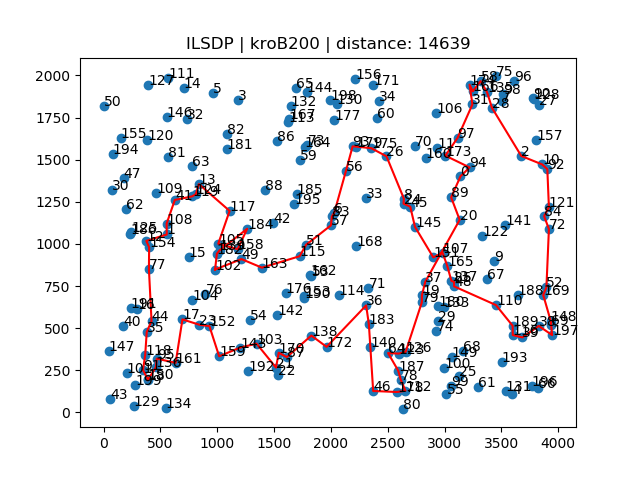
\includegraphics[width=\textwidth]{ilsdp_kroB200.png}
  \end{minipage}
\end{figure}

\begin{figure}[h!]
    \centering
  \begin{minipage}[b]{0.8\textwidth}
    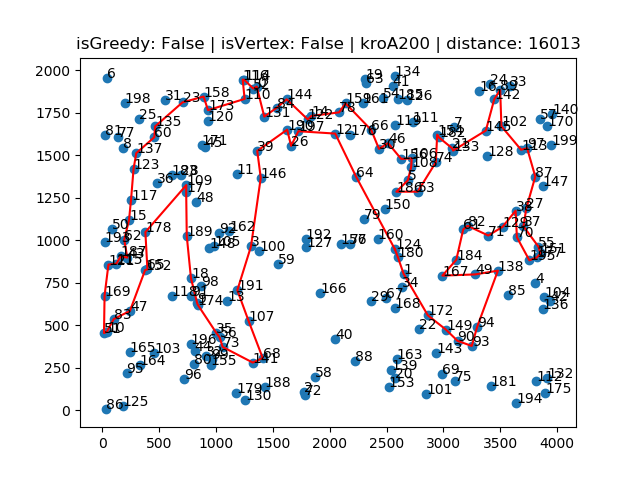
\includegraphics[width=\textwidth]{random_kroA200_V-False_G-False.png}
  \end{minipage}

  \begin{minipage}[b]{0.8\textwidth}
    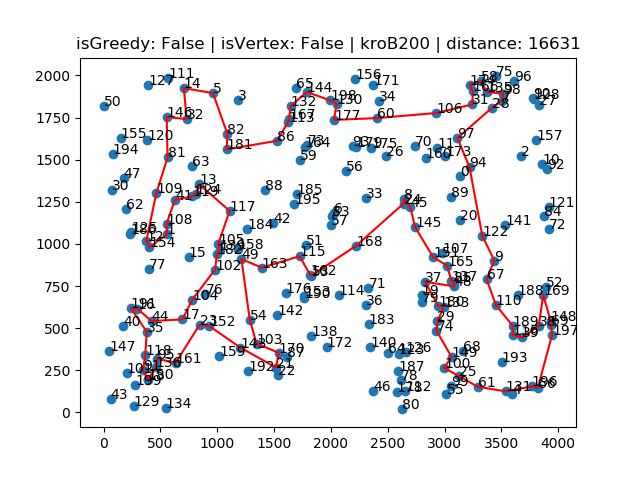
\includegraphics[width=\textwidth]{random_kroB200_V-False_G-False.png}
  \end{minipage}
\end{figure}

\begin{figure}[h!]
  \centering
  \begin{minipage}[b]{0.8\textwidth}
    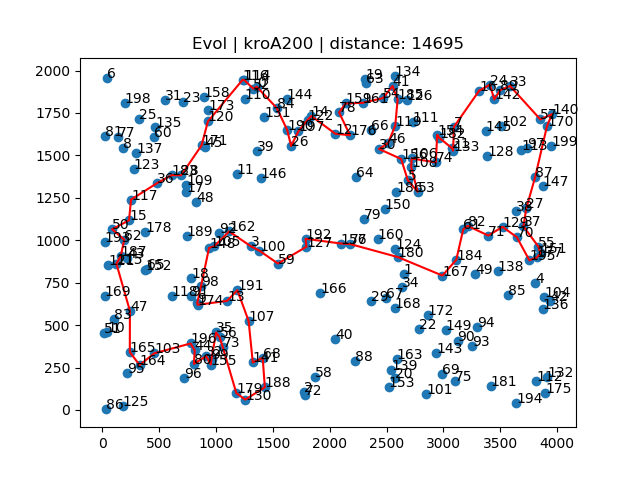
\includegraphics[width=\textwidth]{Evol_kroA200.png}
  \end{minipage}

  \begin{minipage}[b]{0.8\textwidth}
    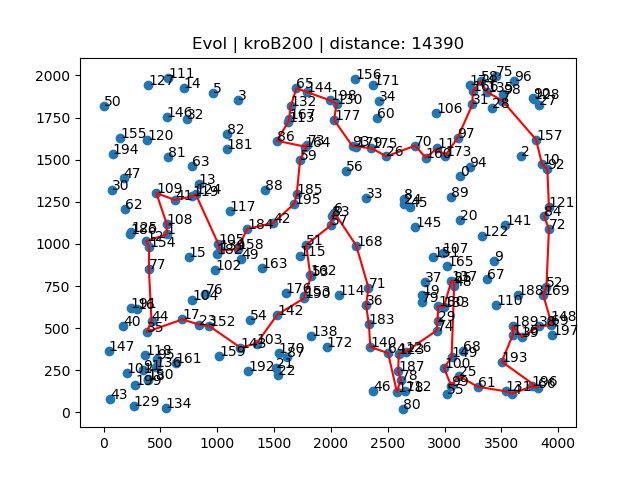
\includegraphics[width=\textwidth]{Evol_kroB200.png}
  \end{minipage}
  
\end{figure}


\section{Wnioski}

Z tabeli wyników można odczytać, że metody Iterated Local Seach dają lepsze wyniki niż metoda Multiple Start Local Search. Czas wykonywania po stronie ILS jest lepszy oczywiście dlatego, że w metodzie MLS zazwyczaj lokalnie przeszukujemy w pełni losowego rozwiązania. Jednakże w porównaniu do poprzednich metod czasy wykonywania zwiększyły się znacząco. Metoda ILS2 z naprawą rozwiązania okazała się nieco bardziej skuteczna od metody w której wymienialiśmy X wierzchołków. 

Hybrydowy algorytm genetyczny poprawia wyniki - szczególnie w przypadku MSLS wynik jest znacząco lepszy. W zależności od instancji (KROA/KROB) wynik jest też lepszy od algorytmów ILS, aczkolwiek raczej zbliżony do ILS2 (DR). Przy zmianach w algorytmie ewolucyjnym jak np. zwiększenie liczby perturbacji oraz znaczące zwiększenie populacji (o 100\%), algorytm ten zaczyna osiagać gorsze wyniki. \textbf{Wynikać to może również z tego, że nasze poprzednie implementacje ILS miały teoretycznie gorsze wyniki niż podobne metody zaimplementowane przez inne grupy, wiec łatwiej było uzyskać poprawę.} 


\section{Kod programu}

    Repozytorium z kodem algorytmów dostępne jest pod: \url{https://github.com/bbbrtk/aem}


\end{document}
